\subsection{Entorno de pruebas}

Para comprobar cómo se ajusta el modelo al comportamiento real de la emisión se tomaron medidas en el Laboratorio de Robótica 0L3 del Instituto de Computación Científica Avanzada de la Universidad de Extremadura (ICCAEx), situado en los Institutos Universitarios de Investigación de la Universidad de Extremadura en Badajoz.

En este laboratorio se dispone de una superficie amplia en la que fue posible usar un robot para automatizar la toma de medidas en divesos puntos, que más tarde fueron usados en la simulación colocando los receptores en dichos puntos.

\begin{figure}[H]
    \begin{subfigure}[b]{.45\textwidth}
      \centering
      \def\svgwidth{0.6\linewidth}
	    \input{./fig/lab.pdf_tex} 
      \caption{Puntos a evaluar}
      \label{fig:puntos}
    \end{subfigure}
    \begin{subfigure}[b]{.45\textwidth}
        \centering
        \def\svgwidth{0.6\linewidth}
	    \input{./fig/lab_vertical.pdf_tex} 
        \caption{Trayectoria en vertical}
        \label{fig:vertical}
      \end{subfigure}
    \caption{Puntos de medida por el robot en el laboratorio y la trayectoria tomada.}
    \label{fig:laboratorio}
\end{figure}

La Figura~\ref{fig:laboratorio} recoge la disposición de los puntos tomados y la ruta del robot para ello.
En total se compone de 35 puntos en los el robot se para y toma medidas cada 5 segundos.

Esta trayectoria se repitió unas 20 veces de modo que fue posible hacer estimaciones sobre todos los puntos con un mayor volumen de datos que pudiera eliminar los efectos de otras redes del edificio.

\subsection{Robot}

Con el fin de automatizar la toma de medidas para hacerla lo más eficiente posible se ha decidido usar un robot móvil capaz de desplazarse mediante navegación autónoma en un entorno conocido.

El elegido en este caso fue el robot TurtleBot 2, un robot con fines educativos y de investigación capaz de desplazarse y orientarse con total libertad en superficies llanas, como eran los en el que se desarrolló este trabajo.
En la Figura~\ref{fig:robot} se puede ver el robot durante una de las tomas de medidas.

\begin{figure}[H]
    \centering
    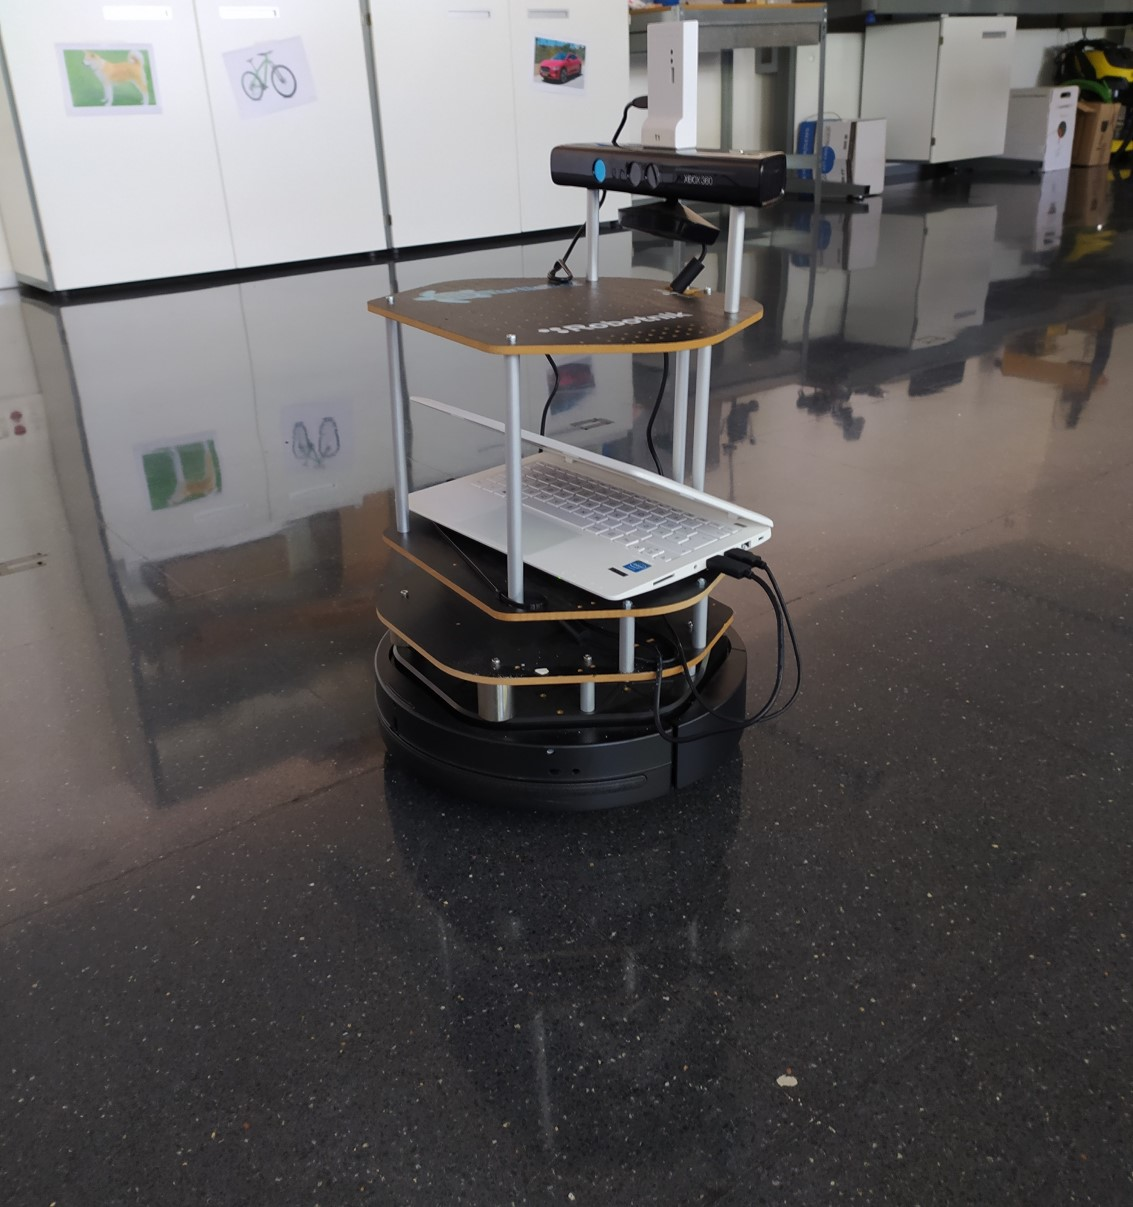
\includegraphics[width=0.55\textwidth]{pic/robot_lab.jpg}
    \caption{Turtlebot en una de las tomas de medidas.}
    \label{fig:robot}
\end{figure}

El TurtleBot funciona con ROS --\textit{Robot Operating System}, en inglés--, un entorno de trabajo enfocado a los sistemas robóticos encargado del soporte para todos los dispositivos hardware del robot como motores, encoders o cámaras. 
Cuenta con diversas librerías para distintos casos de uso, entre las que se encuentra la navegación en un entorno controlado como la que se da en el caso de este trabajo.

Su funcionamiento se basa en una arquitectura de grafos, donde se definen \textit{nodos}, tareas en las que se realiza el procesamiento de sensores, control, actuadores o cualquier otra función.
Los nodos se comunican entre ellos con mensajes llamados \textit{topic}, y es posible su desarrollo con los lenguajes C++ y Python.

Dentro de los paquetes disponibles, el usado en el desarrollo del trabajo es el encargado de la navegación del robot, que permite desplazar al robot a cualquier punto del entorno de trabajo y proporcionar de forma constante su posición en el mapa.

Es posible acoplar al robot un sistema de visión llamado Kinect que, mediante luz, permite obtener un mapa de profundidad del entorno que lo rodea.
Fue desarrollado en primera instancia para el uso en videojuegos pero su uso también se ha extendido a labores de investigación al permitir el posicionamiento de objetos y paredes, de tal manera que permite al robot evitar obstáculos dinámicos en el caso de que interpongan en su camino.

La funcionalidad de navegación aprovecha estos sensores realizando una fusión de sus resultados con los datos de movimiento de los motores que impulsan al robot, de tal forma que es posible corregir cualquier error en casos donde el empuje de las ruedas no se traslade directamente en un desplazamiento del robot, como puede ocurrir al rotar sobre sí mismo.

Para conseguir el posicionamiento en el mapa el paquete de navegación utiliza un \textit{planner} global sobre el que es posible determinar las rutas a seguir por el robot para llegar a un punto dado sorteando obstáculos y paredes.
Junto a él trabaja un \textit{planner} local, en el que gracias a los sensores incorporados se evalúan de forma continua los alrededores del robot.
Así, es posible conseguir de forma continua una evaluación de los posibles obstáculos que no se encuentran en el mapa del planner global, para lo que se construye un mapa de costes con el fin de abortar el movimiento en el caso de que sea imposible alcanzar el punto objetivo \cite{ROSDoc}.

Con la información actualizada del \textit{planner} local, el \textit{planner} global es capaz de modificar los trayectos para que el robot pueda continuar su desplazamiento por el mapa.
Es posible observar un esquema del funcionamiento de estos sistemas en la Figura~\ref{fig:move_base}.

\begin{figure}[H]
    \centering
    \def\svgwidth{0.8\linewidth}
    \input{./fig/navigation.pdf_tex}
	\caption{Esquema del funcionamiento del paquete de navegación de ROS.}
    \label{fig:move_base}
\end{figure}

Con esta herramienta la librería de navegación permite un mapeado autónomo tomando como referencia los datos de odometría que proporcionan los motores propulsores del robot para determinar las dimensiones del entorno.

En el caso de disponer de antemano de dichas dimensiones es posible proporcionar un mapa al sistema de navegación y evitar el paso de reconocimiento del entorno.
Esto no solo ahorra tiempo, sino que además minimiza las posibles discrepancias entre los datos de odometría y los desplazamientos reales del robot al realizar el mapeado de forma autónoma.

La opción de realizar un mapa previo fue la elegida en este caso, ya que el robot cuenta con rutinas para el reposicionamiento en el mapa en dicho caso.
Así, a partir de los límites establecidos y comprobados de forma manual, las posibles discrepancias en la odometría del robot se ven continuamente compensadas y corregidas.

A partir de estos datos corregidos es posible conocer en cualquier momento la posición del robot en el mapa, expuesta a través de ROS en uno de los topic disponibles.

Para facilitar el uso de ROS existe la posibilidad de usar el simulador Stage, capaz de crear un mundo virtual a partir de un mapa en dos dimensiones en el que colocar el Turtlebot y simular su funcionamiento de forma total sin tener acceso al robot de forma física.
Es posible observar su interfaz en la Figura~\ref{fig:stage_rviz}.

Además, ROS también permite el uso de una herramienta de visualización de la posición del robot en el mapa y de todos los sensores que incorpora llamada \textit{rviz}.
Aunque es compatible con Stage, sus funcionalidades brillan al usar el robot en entornos reales, donde es posible comprobar de forma continua que su posicionamiento es correcto y que sus sensores funcionan como es debido.

\begin{figure}[H] 
    \centering
    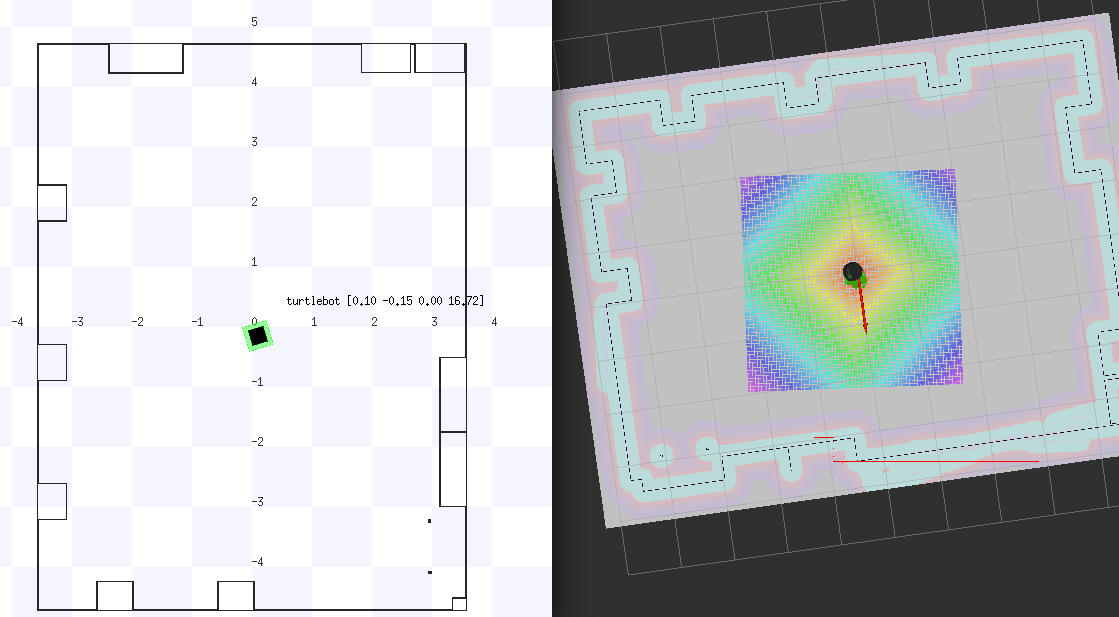
\includegraphics[width=0.75\textwidth]{pic/Stage-rviz.png}
    \caption{Captura del simulador Stage (a la izquierda) y la herramienta de visualización \textit{rviz} (a la derecha).}
    \label{fig:stage_rviz}
\end{figure}
